\documentclass[aps,prl,reprint,10pt,amsmath,amssymb,superscriptaddress,a4paper]{revtex4-2}
\usepackage[utf8]{inputenc} % dding UNICODE support
\usepackage[english]{babel}
\usepackage{indentfirst} % Indentation always (personal preference)
\usepackage{hyperref} % Hyper link for everything
\usepackage{graphicx} % Graphics package
\usepackage{dcolumn} % Double column package
\usepackage{amsmath, amsfonts, amsthm, physics} % Maths packages
\usepackage[margin=2cm]{geometry} % Sets 2cm margins
\usepackage{datetime} % Package for automatic date & time
\usepackage{lipsum} % Inserts dummy latin text into template -- Can remove from final submission
\usepackage{natbib} % Actually using a package to cite unlike the boomers
\usepackage{listings} % To list code in your lab report
\usepackage{appendix} % This one kinda explains itself
\usepackage{xcolor}

\definecolor{codegreen}{rgb}{0,0.6,0}
\definecolor{codegray}{rgb}{0.5,0.5,0.5}
\definecolor{codepurple}{rgb}{0.58,0,0.82}
\definecolor{backcolour}{rgb}{0.95,0.95,0.92}

\lstdefinestyle{mystyle}{
    backgroundcolor=\color{backcolour},   
    commentstyle=\color{codegreen},
    keywordstyle=\color{magenta},
    numberstyle=\tiny\color{codegray},
    stringstyle=\color{codepurple},
    basicstyle=\ttfamily\footnotesize,
    breakatwhitespace=false,         
    breaklines=true,                 
    captionpos=b,                    
    keepspaces=true,                 
    numbers=left,                    
    numbersep=5pt,                  
    showspaces=false,                
    showstringspaces=false,
    showtabs=false,                  
    tabsize=2
}
%%%%%%%%%%%%%%%%%%%%%%%%%%%%%%%%%%%%%%%%%%%%%%%%%%%%%%%%%%%%%%%%%%%%%%%%%%%%%%%%%%%%%%%%%%%%%%%%%%%%%%%%%%%%%%%%%%%%%%%%%%%%%%%%%%%%%%%%%%%%%%%%%%%%%%%%%%%%%%%%%%%%%%%%%%%%%%%%%%%%%%%%%%%%%%%%%%%%%%%%%%%%%%%%%%%%%%%%%%%%%%%%%%%%%%%%%%%%%%%%%%%%%%%%%%%%%%%%%%%%%%%%

\lstset{style=mystyle}
\setcitestyle{authoryear,round}
\begin{document}
\title{Joey's Lab Report Template}
\author{J. Liang (z1234567)}
\affiliation{Cohort A - Mon 9-12 class}
\affiliation{Word count: XXXX words} % If you use VS code like me, this environment is highly recommended: https://marketplace.visualstudio.com/items?itemName=geoffkaile.latex-count

\date{\currenttime~\today}

\begin{abstract}
I would have a succinct (1-2 sentence statement) of the aim in here. And then I would also have a succinct (1-2 sentence statement) of the key conclusion. That is all, keep it simple, it's so a reader can quickly get at your two key points.
\end{abstract}

\maketitle
% You start your main text after here.

\section{Introduction}
This is where I would have some discussion of the general background of your experiment. What are the basic ideas of the topic? What is the question you are setting out to address with this experiment? What are the key underpinning theoretical or experimental results you build on? The assumed knowledge should not exceed the level of a fellow student in your class. Citations to references should be included, and using the literature well is encouraged.

\lipsum[1] % Dummy text
Hello, here's a citation~\citep{Smith:2013jd}, and a little split off equation:

\begin{equation}
\label{eqn1}
E = mc^2
\end{equation}

\begin{figure*}
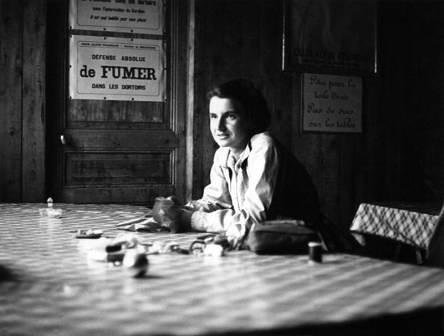
\includegraphics[width = 16 cm]{physicist}
\caption{Doing a full width figure.}
\end{figure*}

\lipsum[2] % Dummy text

Here's how to fit in a huge equation if you wanna, and another cite~\citep{Smith:2012qr}:

\begin{widetext}
\begin{eqnarray}
\label{eqn2} I_{o} = \sin^{2}\left(\frac{2\pi}{\lambda_{\text{ex}}}\Bigl(n_{o}(z_{o}-z_{p})+n_{w}h_{o}\Bigr)\right)\sin^{2}\left(\frac{2\pi}{\lambda_{\text{em}}}\Bigl(n_{o}(z_{o}-z_{p})+n_{w}h_{o}\Bigr)\right) \\
\label{eqn3} I_{p} = \sin^{2}\left(\frac{2\pi}{\lambda_{\text{ex}}}\Bigl(n_{o}z_{o}+n_{w}h_{o}\Bigr)\right)\sin^{2}\left(\frac{2\pi}{\lambda_{\text{em}}}\Bigl(n_{o}z_{o}+n_{w}h_{o}\Bigr)\right)
\end{eqnarray}
\end{widetext}

\lipsum[3] % Dummy text

\section{Aim}

This should be a succinct (1-2 sentence) statement of the aim of the experiment in your report. It does not need to match the lab documentation necessarily, it should be tailored to what you have chosen to focus on in your report and fit well to your conclusion. It should be similar to (or even match) the aim you state in your abstract.

\section{Method}

Should briefly summarise the key aspects of the experiment; the lab documentation can be used as references. In particular, it should note any aspects that differ or are not obvious in the lab documentation.

\lipsum[4] % Dummy text

\section{Results \& Analysis}

Should focus on the key aspects of your results and analysis. It does not need to be exhaustive; you can include a pdf scan of your experiment logbook notes as supplementary material in your final submission if you wish. That said, it should tell a clear story, connect well to the figures that you present, and sensibly justify your final conclusion. Any figure that appears in the results section should be explicitly discussed as part of the results; simply dumping figures onto the page is not good form.

\lipsum[5] % Dummy text

Suppose you want to make a list:\\

\noindent i) First item.\\

\noindent ii) Second item.\\

\noindent iii) Third item.\\

\lipsum[6] % Dummy text

\lipsum[7] % Dummy text

\begin{figure}
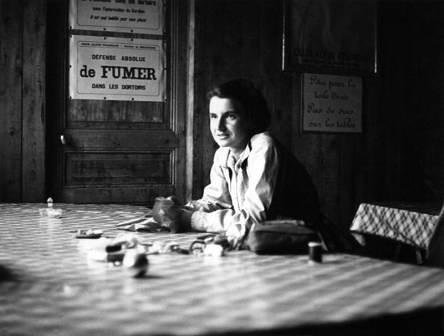
\includegraphics[width = 8 cm]{physicist}
\caption{Schematic illustrating a famous physicist.}
\end{figure}

\lipsum[8] % Dummy text

\section{Discussion}

If you would like this as a section, feel free. This might be a place to distill your analysis down to some key points or make an argument with that analysis.\cite{Other:2014ab}

\lipsum[9] % Dummy text

\lipsum[10] % Dummy text

\section{Conclusions}

You should finish with a succinct (1-2 sentence) statement of your key finding. It should be similar to (or even match) the conclusion you state in your abstract.

\section{Acknowledgements}

The original template of this lab report was put together by Prof. A. P. Micolich from School of Physics, UNSW.

\bibliographystyle{agsm}
\bibliography{sample.bib}

\newpage
\onecolumngrid
\section{\appendixname}
The following is an example of a piece of Python code that will crash your computer
\lstinputlisting{helloworld.py}

\end{document}
